\documentclass[compress,xcolor=table]{beamer}

% Packages
\usepackage[english]{babel}
\usepackage[utf8]{inputenc}
\usepackage[T1]{fontenc}
\usepackage{datetime}

\usepackage{subcaption}
\usepackage{tabularx}
\usepackage{minted}

\usepackage{algorithm}
\usepackage{algorithmic}
\usepackage{amstext} % for \text macro
\usepackage{array}   % for \newcolumntype macro
\newcolumntype{C}{>{$}c<{$}} % math-mode version of "c" column type

% Possible options of the package (add/remove below in \usetheme call):
%  - nosectionpages: no pages between sections
%  - flama: use flama font, requires xelatex/lualatex + the font to compile
%  - compressminiframes: put the heading list bullets indications pages on 1 line
\usetheme[compressminiframes]{sorbonne}

% Title page
\title{LDLt factorization in CUDA}
% \foottitle{SCD gi} % optional, printed at the bottom of the slides, by default same as title, can be useful to rewrite when title has a newline for example
\subtitle{for systems solving} % optional subtitle
\date{\formatdate{22}{03}{2020}}
\author{Maxime \textsc{Darrin} \and Pierre \textsc{Guetschel}}
\institute{M2A - Sorbonne Université} % Optional

% Biblatex
% \usepackage[backend=bibtex, style=authoryear, citestyle=authoryear]{biblatex}

%%%%
%% BEGIN OF SLIDES
%%%%

\begin{document}

\begin{frame}[plain]
	\titlepage
\end{frame}

\section{Our project} \subsection{}

\begin{frame}
	
	\begin{block}{The project}
		We build our project in two parts:
		\begin{enumerate}
			\item The factorization algorithm
			\item The solver (using a factorized form)
		\end{enumerate}
	\end{block}

	\begin{exampleblock}{Hardware}
		Our experiments have been conducted on a GTX 1060 for laptop.
	\end{exampleblock}

\end{frame}



\section{Data storage}

\begin{frame}{}
	Storage of $n$ matrix of size $d*d$

	Matrices $L$ and $D$ :
	\begin{tabular}{|C|C|C|C||C|C|C|C|C|C||C}
		\hline
		D^1_{1,1} & D^1_{2,2} & \dots & D^1_{d,d} & L^1_{1,1} & L^1_{2,1} &
		\dots & L^1_{d,1} & \dots & L^1_{d,d} & \dots\\
		\hline
	\end{tabular}
	\begin{tabular}{C|C|C|}
		\hline
		\dots D^2_{1,1} &  \dots & L^n_{d,d} \\
		\hline
	\end{tabular}

	Matrix $A$ :
	\begin{tabular}{|C|C|C|C||C|C|C|C|C|C||C}
		\hline
		A^1_{1,1} & A^1_{2,2} & \dots & A^1_{d,d} & \emptyset & A^1_{2,1} &
		\dots & A^1_{d,1} & \dots & \emptyset & \dots\\
		\hline
	\end{tabular}
	\begin{tabular}{C|C|C|}
		\hline
		\dots A^2_{1,1} &  \dots & \emptyset \\
		\hline
	\end{tabular}

	with $M^k_{i,j}$ being the element $(i,j)$ of the $k^{th}$ matrix $M$.

	We choosed to store the diagonal elements of $L$ to simplify our code.

	This confguration allows us to compute the factorization in place.
\end{frame}


\section{The factorization}

\begin{frame}{}
	
	\begin{figure}
		\begin{tabular}{c|c|c|c}
			& Max Col & Max k (row) & row + shared memory
			\\
			\hline
			Execution time & 1.489760 ms & 1.487296 m ms & 0.514624  \\
		\end{tabular}
	
	\caption{Comparison on small matrices. (100 matrices of size 32x32)}
	\end{figure}

\end{frame}

\begin{frame}{}
	
	\begin{figure}
		\begin{tabular}{c|c|c}
			& Max Col & Max k (row) 
			\\
			\hline
			Execution time &  1106.73 ms ms & 1108.9 ms \\
		\end{tabular}
		
		\caption{Comparison on large matrices. (100 matrices of size 512x512)}
	\end{figure}
	
\end{frame}

\begin{frame}{Error propagation}
	\begin{figure}
		\centering
		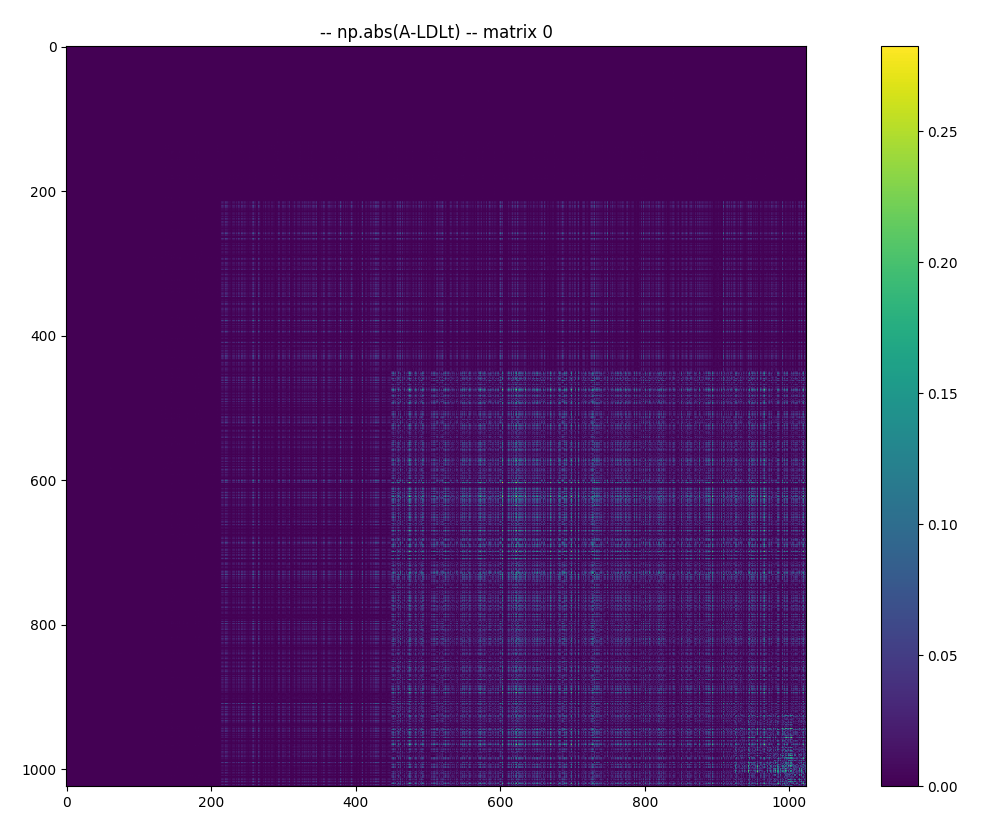
\includegraphics[scale=0.3]{images/bigerrors.png}
		\caption{Error propagation on a big matrice}
	\end{figure}
\end{frame}

\section{The solver}

\begin{frame}{}
	
	\begin{figure}
		\begin{tabular}{c|c|c|c}
			d = & 16 & 128 & 512  
			\\
			\hline
			Execution time &  0.084 ms & 0.960 ms &  12.50 ms \\
		\end{tabular}
		
		\caption{Comparison with 128 threads and 100 matrices (on per block)}
	\end{figure}
	
\end{frame}

\begin{frame}{}

\begin{block}{Behavior}
	We have a gain of time which is linear in the number of threads.
\end{block}
	
\end{frame}

\section{The full pipeline}
\begin{frame}
	\begin{figure}
	\centering
	\begin{tabular}{c|c|c|c}
		& Max Col & Max k (row) & row + shared memory \\
		\hline
		Execution time & 1108.7ms &  1163.1 ms & 0.0091 ms  \\
		Solving time & 13.9 ms & 13.9 ms & 13.9 ms \\		
	\end{tabular}
	
	\caption{Comparison on large matrices. (100 matrices of size 512x512)}
\end{figure}
\end{frame}


\begin{frame}{The end}
	\begin{figure}
		\centering
		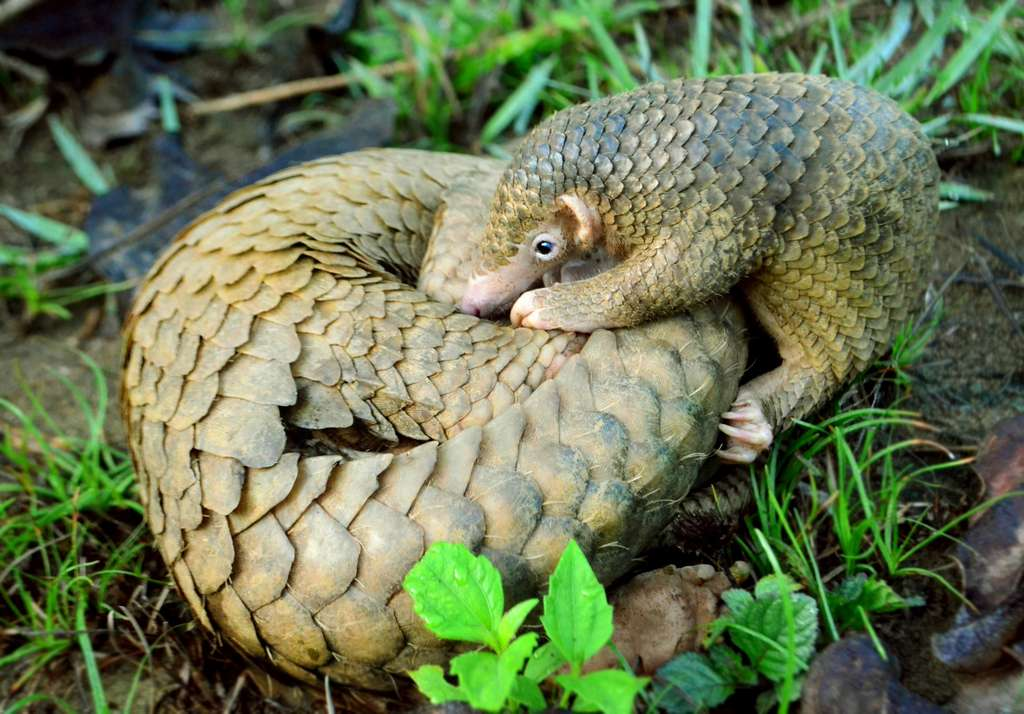
\includegraphics[scale=0.25]{images/pangolin.jpg}
		\caption{A pangolin, probably the source of our current sorrows.}
	\end{figure}
\end{frame}





\end{document}

